\documentclass[11pt]{article}
\usepackage{url} 
\usepackage{graphicx}
\usepackage[margin=1in]{geometry}
\graphicspath{ {img/} } 


\title{\textbf{The Topology of Sleep}}
\author{Vishnu Menon\\  
		John Jeong}
\date{}
\begin{document}

\maketitle

\section{Abstract}
In this report, we describe the results of applying Topological Data Analysis techniques to Polysomnography data (specifically, EEG waveforms). We attempt to use TDA-derived features to train classifiers for two separate Polysomnography-related tasks: identifying sleep spindles and classifying sleep stage. We describe our feature-generation and classification pipeline and consider possible sources of inaccuracy. Then, we evaluate the performance of our classifiers relative to the state-of-the-art and discuss future developments that could increase the accuracy of our approach.
  

\section{Our Dataset}
The National Institute of Neurological Disorders and Stroke estimates that over 60 million people in America alone suffer from sleep-related problems. Of these, at least 40 million suffer from chronic and long-term sleep disorders. Sleep-related medical expenses each year amount to over \$16 billion \cite{ninds}. Diagnosing and studying sleep disorders, therefore, is a major concern for many medical professionals. Polysomnography, the process of carrying out sleep studies, is often a key part of the diagnostic/exploratory process in sleep-related medical cases. A typical polysomnograph (the output of polysomnography) contains, among other signals, a patient's brainwaves, heartbeat, and breathing recorded over the course of a full night's sleep. This wealth of data often requires hours of careful analysis by trained professionals in order to interpret. Two aspects of polysomnograph data that are often measured and annotated are the positions/durations of the sleep stages/phases and the  locations of sleep spindles. 

Human sleep is divided into 5 phases: stages 1,2,3, and 4, and REM (Rapid Eye Movement) sleep. The stages vary in terms of depth of sleep, brain and muscle activity, dream activity, heart rate, and blood pressure (as well as other factors). The amount of time an individual spends in each phase can hint at various underlying issues with his or her sleep patterns; for example, patients with Sleep Apnea are often robbed of REM sleep, leaving them tired and irritable. Each sleep stage comes with distinctive EEG waveforms by which they can be identified, as shown in Figure \ref{fig:stageseeg}.

\begin{figure}[h]
    \centering
    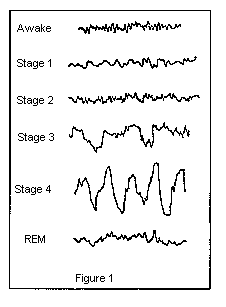
\includegraphics[width=0.25\textwidth]{sleepeeg} 
    \caption{Representative EEG waveforms from each sleep stage \cite{ninds}}
    \label{fig:stageseeg}
\end{figure}

Sleep spindles are EEG events that occur in non-REM sleep. They typically appear as ``waxing-and-waning 10--16 Hz oscillations lasting 0.5–2 s" \cite{Andrillon17821}. There are many hypotheses about their function, including suggestions that they are involved in memory, arousal, and environmental disconnection during sleep. Spindles' characteristics have also been used as an indicator for certain psychiatric disorders (including schizophrenia) \cite{Andrillon17821}.

Due to their medical relevance and their universal nature, both of these types of polysomnograph events (i.e. phases and spindles) are important to sleep specialists studying patient data. To analyze their topological characteristics, we turned to two separate datasets. The first is the DREAMS Sleep Spindle Database. This dataset consists of ``8 excerpts of 30 minutes of central EEG channel (extracted from whole-night [polysomnograph] recordings), annotated independently by two experts in sleep spindles" \cite{dreams}. The excerpts vary in sampling frequency and in EEG channel used. Additionally, only 6 of the excerpts were scored by both experts, so only those 6 were used in this project. The other dataset that we utilized is the PhysioNet Sleep-EDF Database, a ``collection of 61 polysomnograms (PSGs) with accompanying hypnograms (expert annotations of sleep stages) ... from two studies" \cite{kemp2000analysis}. All the EEG data in these polysomnograms is from the Fpz-Cz and Pz-Oz channels/electrode locations, and all of it is sampled at 100Hz. These two channels are used to annotate each polysomnogram with the labels W (Awake), M (Movement), ? (Uncertain), 1, 2, 3, 4, and REM; only the latter 5 labels are used in this project.  

\section{Goals} 

Given these two datasets, we hope to automate the process of identifying spindles and stages through machine learning. With sufficient accuracy, this could be helpful in a variety of medical sleep-related applications. We also hope to attain this accuracy through the use of efficiently computed TDA-based features, to validate the applicability of TDA to this use-case.

\section{Existing Works}
 
There is existing work in both addressing our sleep-related tasks and in applying topology to EEG data, but as far as we could tell, not in our specific use-case. Many researchers already believe that topological analysis provides promising information for discerning various conditions and examining the dissimilarity in graphical EEG features for different experimental groups. For example, a study done by Smith and Escuardo introduced a novel method to analyze brain networks called the Weighted Complex Hierarchy Model (WCH) that probes the complex hierarchical topology of the network to facilitate connectivity research \cite{smith2017complex}. More close to our persistent-homology-driven approach is that of Wang, who's research on epilepsy utilized topological features in the EEG signals before and after a seizure attack \cite{wangtopological}. Tangentially related research done by Babkoff and his team examined the effects of a 72-hour sleep loss by looking at the topology of brain performance curves \cite{babkoff}.

The specific task of identifying sleep spindles suffers from a distinct lack of standardization, since there are many disagreements even between experts about exactly what constitutes a spindle, and a large amount of variance in relevant datasets. Though there have been many attempts at automatic detection (since approximately 1970), the most relevant to us was the research done using the same dataset. The work of Devuyst et al. proposed clear guidelines for evaluation and introduced the dataset that we chose to use \cite{devuyst}. Devuyst used a fairly naive detection algorithm that utilized band-pass filtering and level-detection along with a Bayesian approach. Her work chose to use only the spindles on which both scorers agreed (as did ours), and her algorithm performed with a recall/sensitivity of 70.20\% of the results. She also described other approaches performed on different datasets, including an approach that applied Short Time Fourier Transforms along with linear discriminant analysis to achieve sensitivity of 86\% as well as SVM based models that added adaptive autoregressive modeling to achieve agreement rates of 93-96\% \cite{devuyst}.

The sleep-stage classification task is considerably more well-developed. A 2001 effort by Hanaoka used a process that extracts characteristic parameters from EEG waveforms (i.e. identifies certain types of waves based on direction, peak, bottom, and duration of EEG waves) and trained a decision tree on this data to achieve roughly 70\% accuracy \cite{hanaoka}.  Coincidentally, this is also roughly the agreement percentage between specialists. A more recent project, carried out by Hassan, in 2015, achieved 87--89\% classification accuracy (on the same dataset that we used) by using a decomposition called CEEMDAN and then ``extract[ing] various statistical features from the intrinsic mode functions" \cite{hassan}. These features were then used to train an AdaBoost classification model. We hoped to achieve comparable results with our own classification model. 

\section{Our Methods \& Results}

Our pipelines for Spindle Identification and for Stage Classification ended up being relatively similar. For both tasks, we got the best results using a feature based on sorted persistence values, which we found rather surprising. 

For spindle classification, we initially took the two expert annotations for each polysomnograph excerpt and compared them to find a list of spindle locations/durations that both agreed on. We read the data for each of the spindles using a slightly modified (to account for format errors in our input files) version of the MNE library \cite{mne}. We then picked random locations in the samples that hadn't been identified by \textit{either} expert as being spindles, and read in snippets of lengths randomly drawn from the pool of lengths found in positive samples. We accumulated twice as many negative samples as positive samples. For each sample, we generated a feature by calculating the 0D function persistence of the EEG waveform encapsulated by the sample. We used the $\mu V$ value of the EEG signal as the height function and added the 'edge' between two consecutive points at the height of the higher point. To create the persistence diagram, we used code of our own that removes points that aren't minima or maxima and then keeps track of the component of each point as the height threshold is increased incrementally to record birth and death times. During this process, we removed every other point to provide a rough smoothing, to account for noise in the EEG signal. This step proved especially important because of the varying frequencies of the data. After we generated the persistence diagram, we calculated the persistences for each point and then returned a vector of these persistences sorted in decreasing order, truncated or zero-padded to be length 40. We found that increasing the size of the feature vector consistently gave us better results, so we chose 40 because in almost all cases it was larger than the size of the list of persistence diagram points.

Once we'd generated these features, we used them to train a variety of machine learning classifiers provided by the scikit-learn toolkit \cite{sklearn}. We split our features at random into 75\% for training and 25\% for testing, and calculated accuracy, precision, and recall for each classifier. Our results are summarized in the table below: 

\begin{figure}[h]
    \centering
    \begin{tabular}{|c|c|c|c|}
\hline
	 & Accuracy (\%) & Precision (\%) & Recall (\%) \\
\hline
	Nearest Neighbors (k=3) & 0.842 & 0.800 & 0.716\\
\hline
	Linear SVM & 0.871 & 0.920 & 0.676\\
\hline
	RBF SVM & 0.663 & 0 & 0\\
\hline
	Poly SVM & 0.851 & 0.913 & 0.618 \\
\hline
	Sigmoid SVM & 0.317 & 0.027 & 0.029\\
\hline
	Decision Tree & 0.871 & 0.800 & 0.823\\
\hline
	Random Forest & 0.861 & 0.857 & 0.705 \\
\hline
	Neural Net & 0.861 & 0.884 & 0.676 \\
\hline
	AdaBoost & 0.851 & 0.852 & 0.676\\
\hline

\end{tabular}

    \caption{Classifier performance for spindle identification}
    \label{fig:spindleresults}
\end{figure}

Decision Trees seemed to consistently give us our best/most balanced results. The performance that we managed with them is definitely short of state-of-the-art, as discussed in the Existing Works section. However, we believe it is still a respectable performance given the very low ``inter-human agreement rate for sleep spindles scoring" \cite{devuyst}, and shows promise for the application of TDA and Persistent Homology to this task. 

Our approach fared somewhat worse at the task of sleep stage classification. We approached it in a similar way; we once again read the input data using MNE and then select two random samples from each annotated event (i.e. each sleep-stage annotation). Sample size was a parameter that we found had a significant impact on accuracy, and 6000 samples (i.e. 60 seconds) proved to offer a good tradeoff between efficiency and accuracy. We discarded any annotated stages that were shorter than our sample size parameter. For each sample, we computed a sliding window point-cloud using the code provided by Dr. Tralie, which we then mean-centered and normalized (we also tried this process without mean-centering and normalization, but there was no significant impact on accuracy). When generating our point-cloud, we used a vector embedding dimension of 100,  an increment of 2, and a hop size of 15. We picked these values mostly through trial and error, though our embedding dimension was roughly based on the idea, gained through inspection of waveforms, that the period of more noticeably periodic deep sleep waves was roughly 1--2 seconds. Once we'd created these point clouds, we used Dr. Tralie's Ripser wrapper to generate Rips Filtration persistence diagrams. We chose to only consider 1D persistence, since our approach was based on the varying periodicity and we expected to see this as 'loops' in the Rips Filtration. We used two different approaches to generating features from these persistence diagrams. The first was identical to the one used in spindle detection, except we found that a slightly smaller feature size (30) was more effective. The second was a binning-based approach that split the persistence diagram into a $12 \times 12$ grid and then maintained a count of how many persistence points fell into each. In either case, we prepended the min and max values attained by the signal in the sample to the feature vector; we found this to increase accuracy, because it helped represent the amplitude of the waveform. Since the sleep stage annotations were based on two channels of EEG data (Fpz-Cz and Pz-Oz), for each sample, we carried out this full point-cloud-and-feature-generation process individually on each channel and then simply concatenated the results for our final feature. Once we had generated these features, we again trained and tested an array of classifier types and recorded classification accuracy (i.e. $correct / total$) to evaluate. We initially tested on samples from the same files that we trained with, and got extremely high accuracy (i.e. above 98\% consistently); however, we discovered to our dismay that this was a result of the classifiers learning specific features of the training files and recognizing them in the test samples (especially problematic since our randomly selected samples often overlapped). We then switched to training on a set of files and testing on a different set, using 70\% of files for training. This gave us drastically worse (but still passable) results, as summarized in the following table: 
 
\begin{figure}[h]
    \centering
\begin{tabular}{|c|c|c|}
\hline
	 & Accuracy (\%) with F1 & Accuracy (\%) with F2 \\
\hline
	Nearest Neighbors (k=3) & 0.492 & 0.563 \\
\hline
	Linear SVM & 0.464 & 0.549\\
\hline
	RBF SVM & 0.591 & 0.464\\
\hline
	Poly SVM & 0.464 & 0.591\\
\hline
	Sigmoid SVM & 0.464 & 0.464\\
\hline
	Decision Tree & 0.591 & 0.521\\
\hline
	Random Forest & 0.563 & 0.648\\
\hline
	Neural Net & 0.478 & 0.690\\
\hline
	AdaBoost & 0.560 & 0.478\\
\hline
\end{tabular}
 
    \caption{Classifier performance for stage classification. F1 refers to the first method of feature generation (vector of sorted persistences), while F2 refers to the second (binning)}
    \label{fig:stageresults}
\end{figure}

Surprisingly, there was little appreciable difference between our two methods of feature generation, though the Neural Net with the second feature generation approach was the best performing classifier by a sizable margin at 0.69\%. Across the board, our results were far worse than the state-of-the-art. However, we believe that they do show some promise and that these results in no way show that TDA is poorly suited to the task at hand. In addition, we noticed that many of the more impressive results were from sources that combined stages 3\&4 or took similar steps to simplify the task, which we did not choose to do. 
 
\section{Future Plans}

We believe that a major contributor to our limited success in stage classification is the number of parameters for which we had to choose values (e.g. the sliding-window parameters and the sample size). The values for these parameters were chosen through trial and error, and we have no confidence at all that they are optimal. The TDA approach, especially when attempting to identify periodicity, seems very dependent on choosing these parameters well; with more computing power and time, we would like to vary these parameters more systematically to identify optimal values. Alternatively, we would like to do more research into existing literature on sleep stages to see if there is any evidence supporting certain parameter values. 

Additionally, the fact that our TDA features were not wholly successful but clearly held non-negligible predictive power makes us believe that combining them with other features might be worthwhile. We would like to try adding our TDA features to state-of-the-art features used in this task and see if they can improve accuracy by working in tandem. 

Finally, there are a variety of other TDA feature generation methods that might prove more well-suited to this task, so we would be interested in trying more options to see if we simply haven't found the right one. Regardless, this project has left us with the conviction that TDA has definite value to offer to the tasks of sleep stage classification and sleep spindle identification.\\
\\
All code referenced in this report can be found at \url{https://github.com/vishnumenon/SleepTopology}

\bibliography{bibliography} 
\bibliographystyle{acm}


\end{document}
